\documentclass[12pt,a4paper]{book}

\usepackage[utf8]{inputenc}
\usepackage[table,dvipsnames]{xcolor}
\usepackage[english]{babel}
\usepackage{newlfont}
%font
\usepackage{tgcursor}
\usepackage{tgpagella}
%force line break in cell
\usepackage{makecell}
\usepackage{caption,rotating}
\usepackage{subfigure}
\usepackage{pdflscape}
\usepackage{graphicx}
\usepackage[parfill]{parskip}
\usepackage[labelfont=bf]{caption}
%\usepackage{multicol}
\usepackage{hyperref}
\hypersetup{
    colorlinks=false,
    linkcolor=black,
    filecolor=blue,      
    urlcolor=blue,
}

%citation
\usepackage{epigraph}
\usepackage{etoolbox}
    \makeatletter
    \newlength\epitextskip
    \pretocmd{\@epitext}{\em}{}{}
    \apptocmd{\@epitext}{\em}{}{}
    \patchcmd{\epigraph}{\@epitext{#1}\\}{\@epitext{#1}\\[\epitextskip]}{}{}
    \makeatother

    \setlength\epigraphrule{0pt}
    \setlength\epitextskip{2ex}
    \setlength\epigraphwidth{.8\textwidth}

%include images in table
\usepackage{enumitem}
\usepackage{booktabs}

%math symbols
\usepackage{amsthm}
\usepackage{amssymb}
\usepackage{amsmath}
\usepackage{amsfonts}
%\usepackage{multicol}
%\usepackage{ltablex}
%\usepackage{eurosym}
%\usepackage{dcolumn}
\usepackage[margin=2 cm]{geometry}

%biblatex packages
\usepackage[
natbib=true,
backend=biber,
style=apa,
citestyle=authoryear-ibid
]{biblatex}
\setlength\bibitemsep{\baselineskip}
\addbibresource{a-shelves-voyage.bib}

\theoremstyle{definition}
\newtheorem{game}{Game mechanics}[section]
\newtheorem{exam}{Example}[section]
\newtheorem{sugg}{Alternative Rule}[section]
\newtheorem{claim}{Claim}[section]
%\newtheorem{oef}{Exercize}[section]
\newtheorem{rem}{Remark}[section]

\begin{document}
\setcounter{chapter}{1}
\pagenumbering{gobble}

\begin{titlepage}
\begin{center}
\vspace{1cm}
{{\Large{\textsc{Orpheus Instituut \\}}}}
\vspace{1cm}
\begin{figure}[h!]
\begin{center}
\includegraphics[scale=0.8]{./figures/LOGO_Orpheus_Grootgebruik.png}% inserire il logo dal sito dell'universita'
\end{center}
\end{figure}
 %\rule[0.1cm]{15.8cm}{0.1mm}
{\LARGE{\bf Resounding Libraries}}
\end{center}
\vspace{3 mm}
\begin{center}
{\Huge{\bf A Shelves Voyage }}\\
\begin{center}
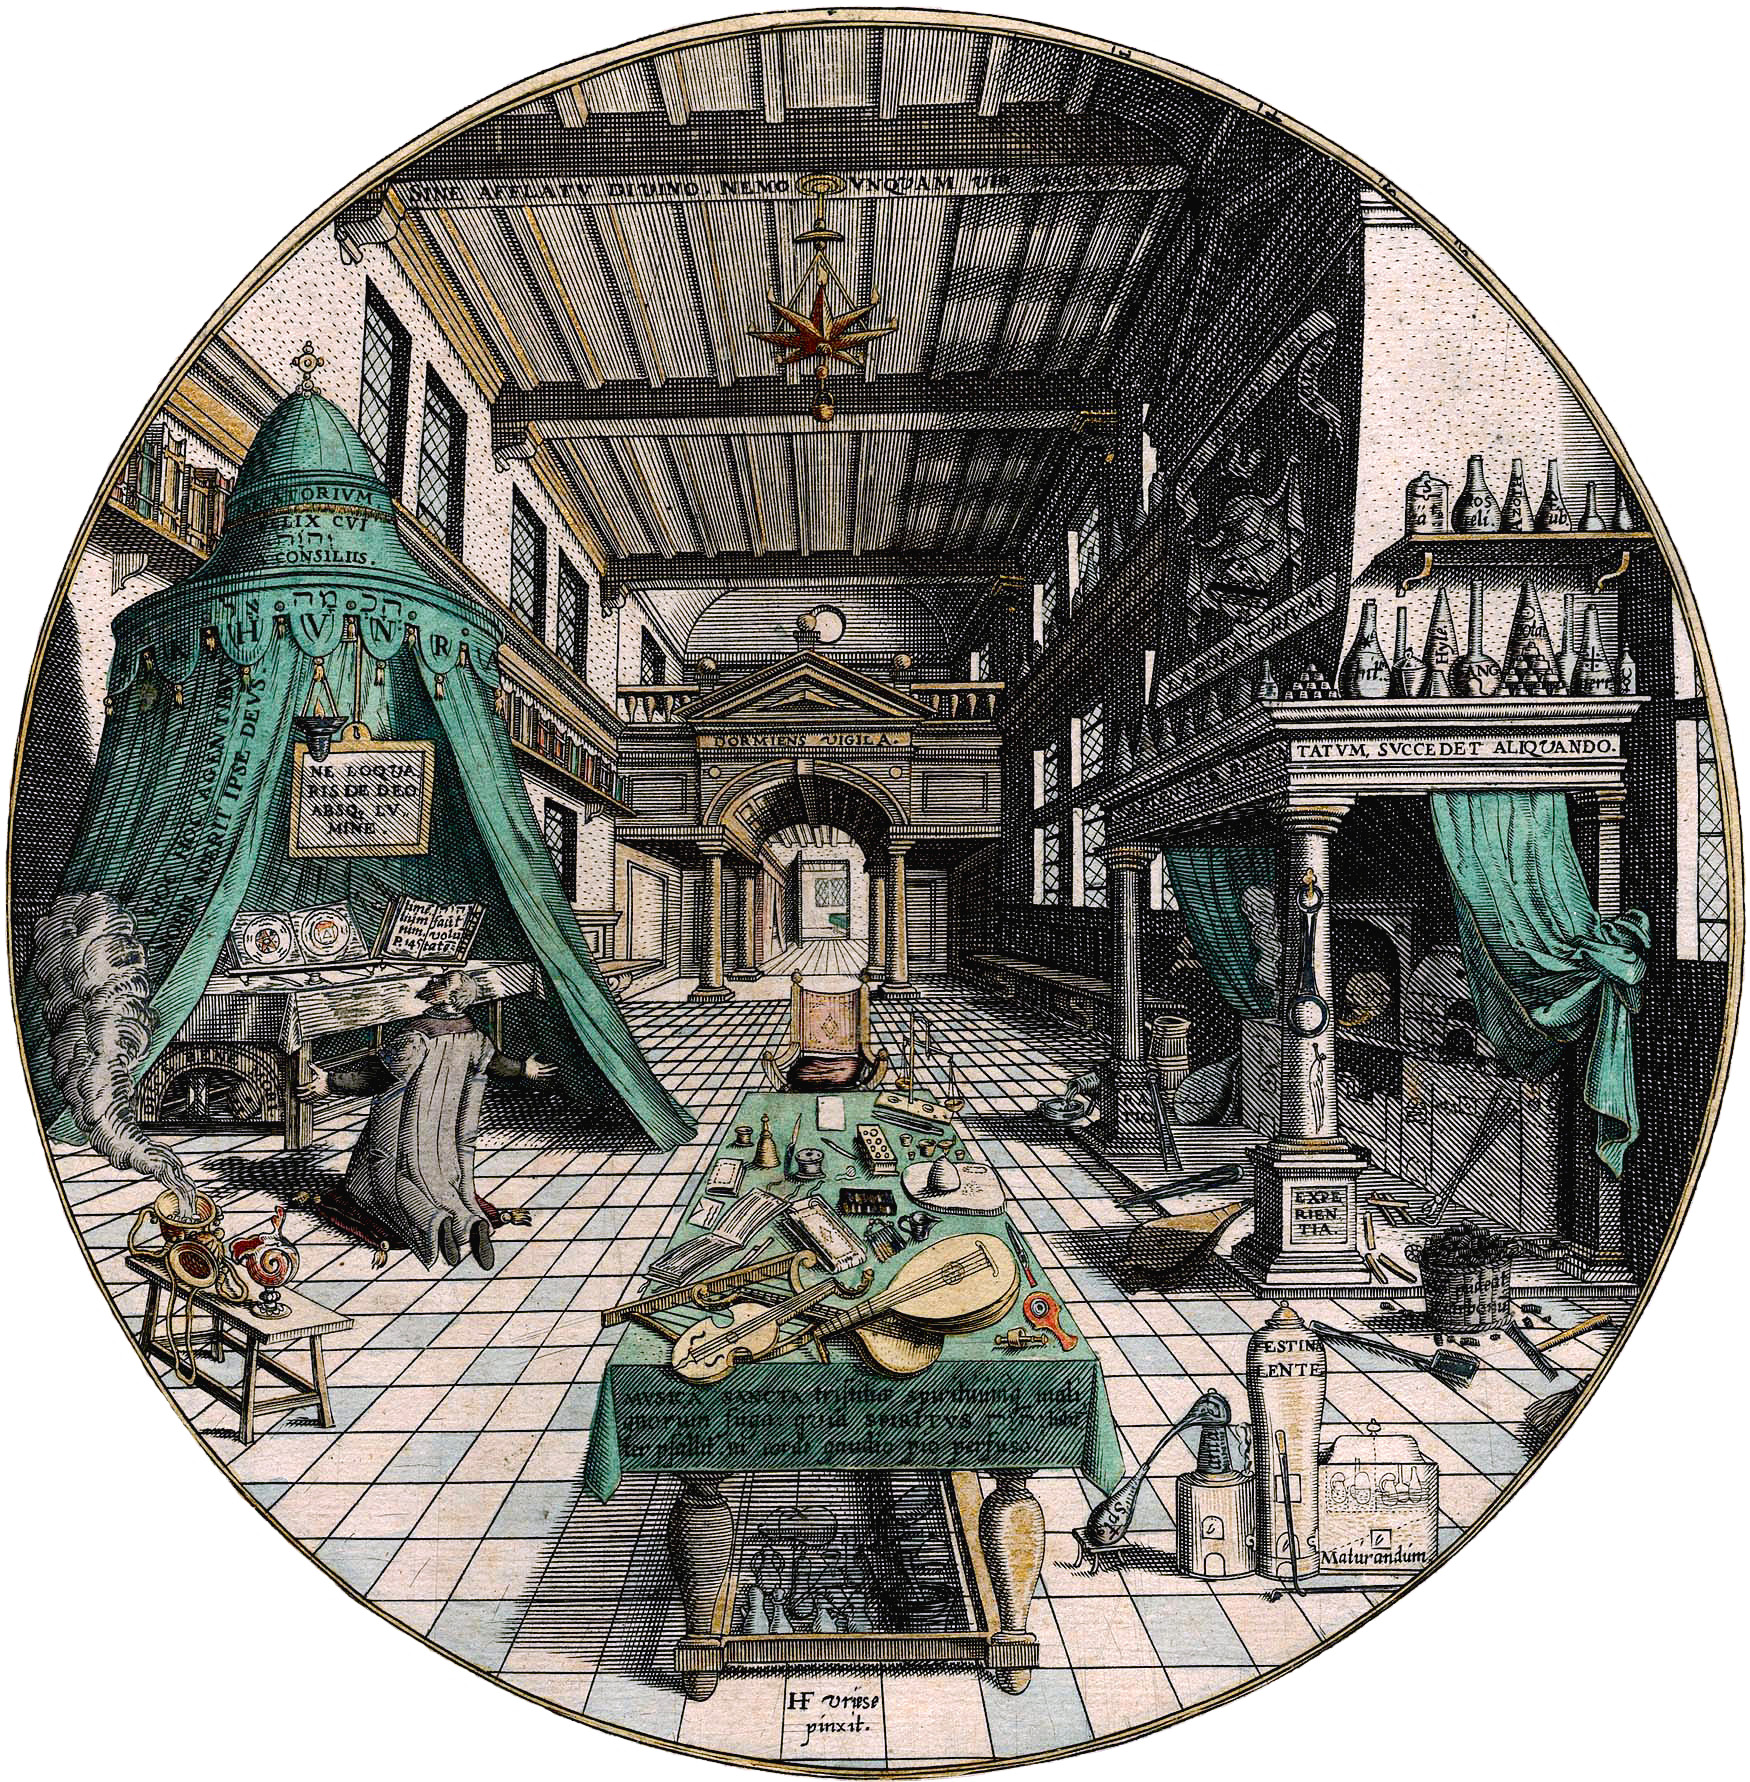
\includegraphics[scale=0.2]{./figures/Pasted image 20240110181553.png}
\end{center}
\vspace{3mm}
{\large{\bf A Game of Imaginary Travels for Researchers and Libriaries }}\\

\end{center}


\end{titlepage}

\newpage
\pagenumbering{roman}
\setcounter{tocdepth}{3}
\tableofcontents
\newpage

\section*{Prologue}

\epigraph{
You can deny, if you like, nearly all
abstractions: justice, beauty, truth, goodness, mind, God. You
can deny seriousness, but not play.}
{Johan Huzinga, \textit{Homo Ludens} (1938)}


\newpage

\pagenumbering{arabic}

\section{Introduction}

\begin{center}
\includegraphics[scale=0.4]{./figures/Pasted image 20240110181353.png}
\end{center}

\subsection{What is the game about?}

\textit{A Shelves Voyage} is a game about \textbf{discovery}, \textbf{plurality}, and \textbf{unexpected journeys} designed for researchers and librarians wishing to unchain the potential of knowledge graphs in their practice.

During a game session, the players are encouraged to reconsider their viewpoint on entities and concepts related to their research field, or catalogue, through a collaborative, and sometimes adversarial, creation of a knowledge graph of entities and properties. 

We have introduced some randomness in the process to drive players outside their intellectual comfort zones, to explore the possibilities of unbeaten tracks, opening to the marvel of possibilities of \textit{ars combinatoria}.  

Furthermore, the game is suited for researchers and librarians willing to think in \textit{semantic triples}, according to the Resource Description Framework (RDF), and explore the possibilities provided by Linked Open Data and knowledge graphs. 

This small game wishes to accustom in a fun and engaging way the ones who dare to understand the potential of these new technologies for the Humanities and the Arts. 

\newpage

\subsection{Objectives}

\begin{center}
\includegraphics[scale=0.25]{./figures/monkeys.jpg}
\end{center}

In his seminal work \textit{Homo Ludens}, Johan Huzinga claims that human culture, from religious practices to art and storytelling, are no more than a game. Through play, humanity regulates itself and allows progress and discovery.

While researching, being it in a conference or informal meeting, we tend to play a specific role, endlessly repeating a part circumscribed within the boundaries of our expertises. We tend to stick to topics and citations we are comfortable with, and as result we betray the initial aim of the conversation: \textbf{communication}. 

Taking inspiration from board, storytelling and role-playing games, we wish to breaking the parroting cycle of scholars and society, opening the possibility to consider the unimaginable and the unusual introducing some randomness in the conversation. 

Through play, interaction, conflict and randomness, the players collaboratively create a knowledge graph of entities (nodes), represented by circular tokens, and properties (edges), made with cords. 

Each game session experience, or \textit{imaginary travel}, through physical or metaphorical shelves, can be adapted to the players' need and aims, thanks to a series of independent game modules. Also, journeys can be easily tied together in longer voyages, spreading out in several gatherings. 

\newpage

\subsection{RDF triples and knowledge graphs}

\begin{center}
\includegraphics[scale=0.35]{./figures/Fludd-De natura simia-II-210.png}
\end{center}

In the last decades, we have experienced a growing interest in organising knowledge on the Web, thanks to Semantic Web technologies and Linked Open Data.
Metadata from different libraries, research institutions and the wide web of Internet are getting structured according to several data models, from tabular data to relational database, passing through XML schema and semantic triples. 

According to the FAIR Data Principles, we believe in \textbf{findable}, \textbf{accessible}, \textbf{interoperable}, and \textbf{reusable} data. The Resource Description Framework (RDF) provides an elegant solution to address the aforementioned issues, linking metadata between several catalogues, ontologies and vocabularies on the Web.

There are several publications available for the not domain experts, like librarians and researchers in the fields of Humanities and Arts, that the reader might refer to for a more technical discourse. This game wishes to contribute to the spreading of FAIR principles in a more ludic and philosophical manner, advocating the human role in knowledge base.

\newpage  

\section{Core mechanics and setup}

\begin{center}
\includegraphics[scale=0.45]{./figures/600px-Boilly-Checkers-1803.jpg}
\end{center}

\subsection{Setting-up the board}

\epigraph{
In the history of ideas, we should consider several dead-end paths, and not only confine ourselves to the main roads.}
{David S. Katz,The Occult Tradition (2005)} 

To play \textit{A Shelves Voyage} you will need to gather \textbf{a group of 2 to 6 players}, willing to explore unexpected paths of knowledge between familiar, and less familiar, concepts.
This game is an ode to the tactile power of \textbf{tabletop games} using analog technologies such as pen-and-paper, meeples and tokens. 

We encourage the players to gather in a quiet and lightly space, preferably a library hall surrounded by endless bookshelves. There is no specific time limit for a game session, or \textit{imaginary travel}, and the game can be adapted to the group's needs thanks to a series of modules, enhancing the experience with additional complexity and depth.

You will need

\begin{itemize}

\item Some pencils and small index cards to record entities and properties names, recording points and special cards and other actions.

\item Some circular disks or tokens, representing the nodes of your knowledge graph.

\item Some small cords and meeples of different colors, one for each player.

\item A poll of six-sided dice (D6s)

\item A deck of Objective cards and Magic Items (optional module)

\item Small tokens symbolising coins players can earn.

\item At least one hour of play.

\end{itemize}

\newpage

\subsection{Game Phases}

\begin{center}
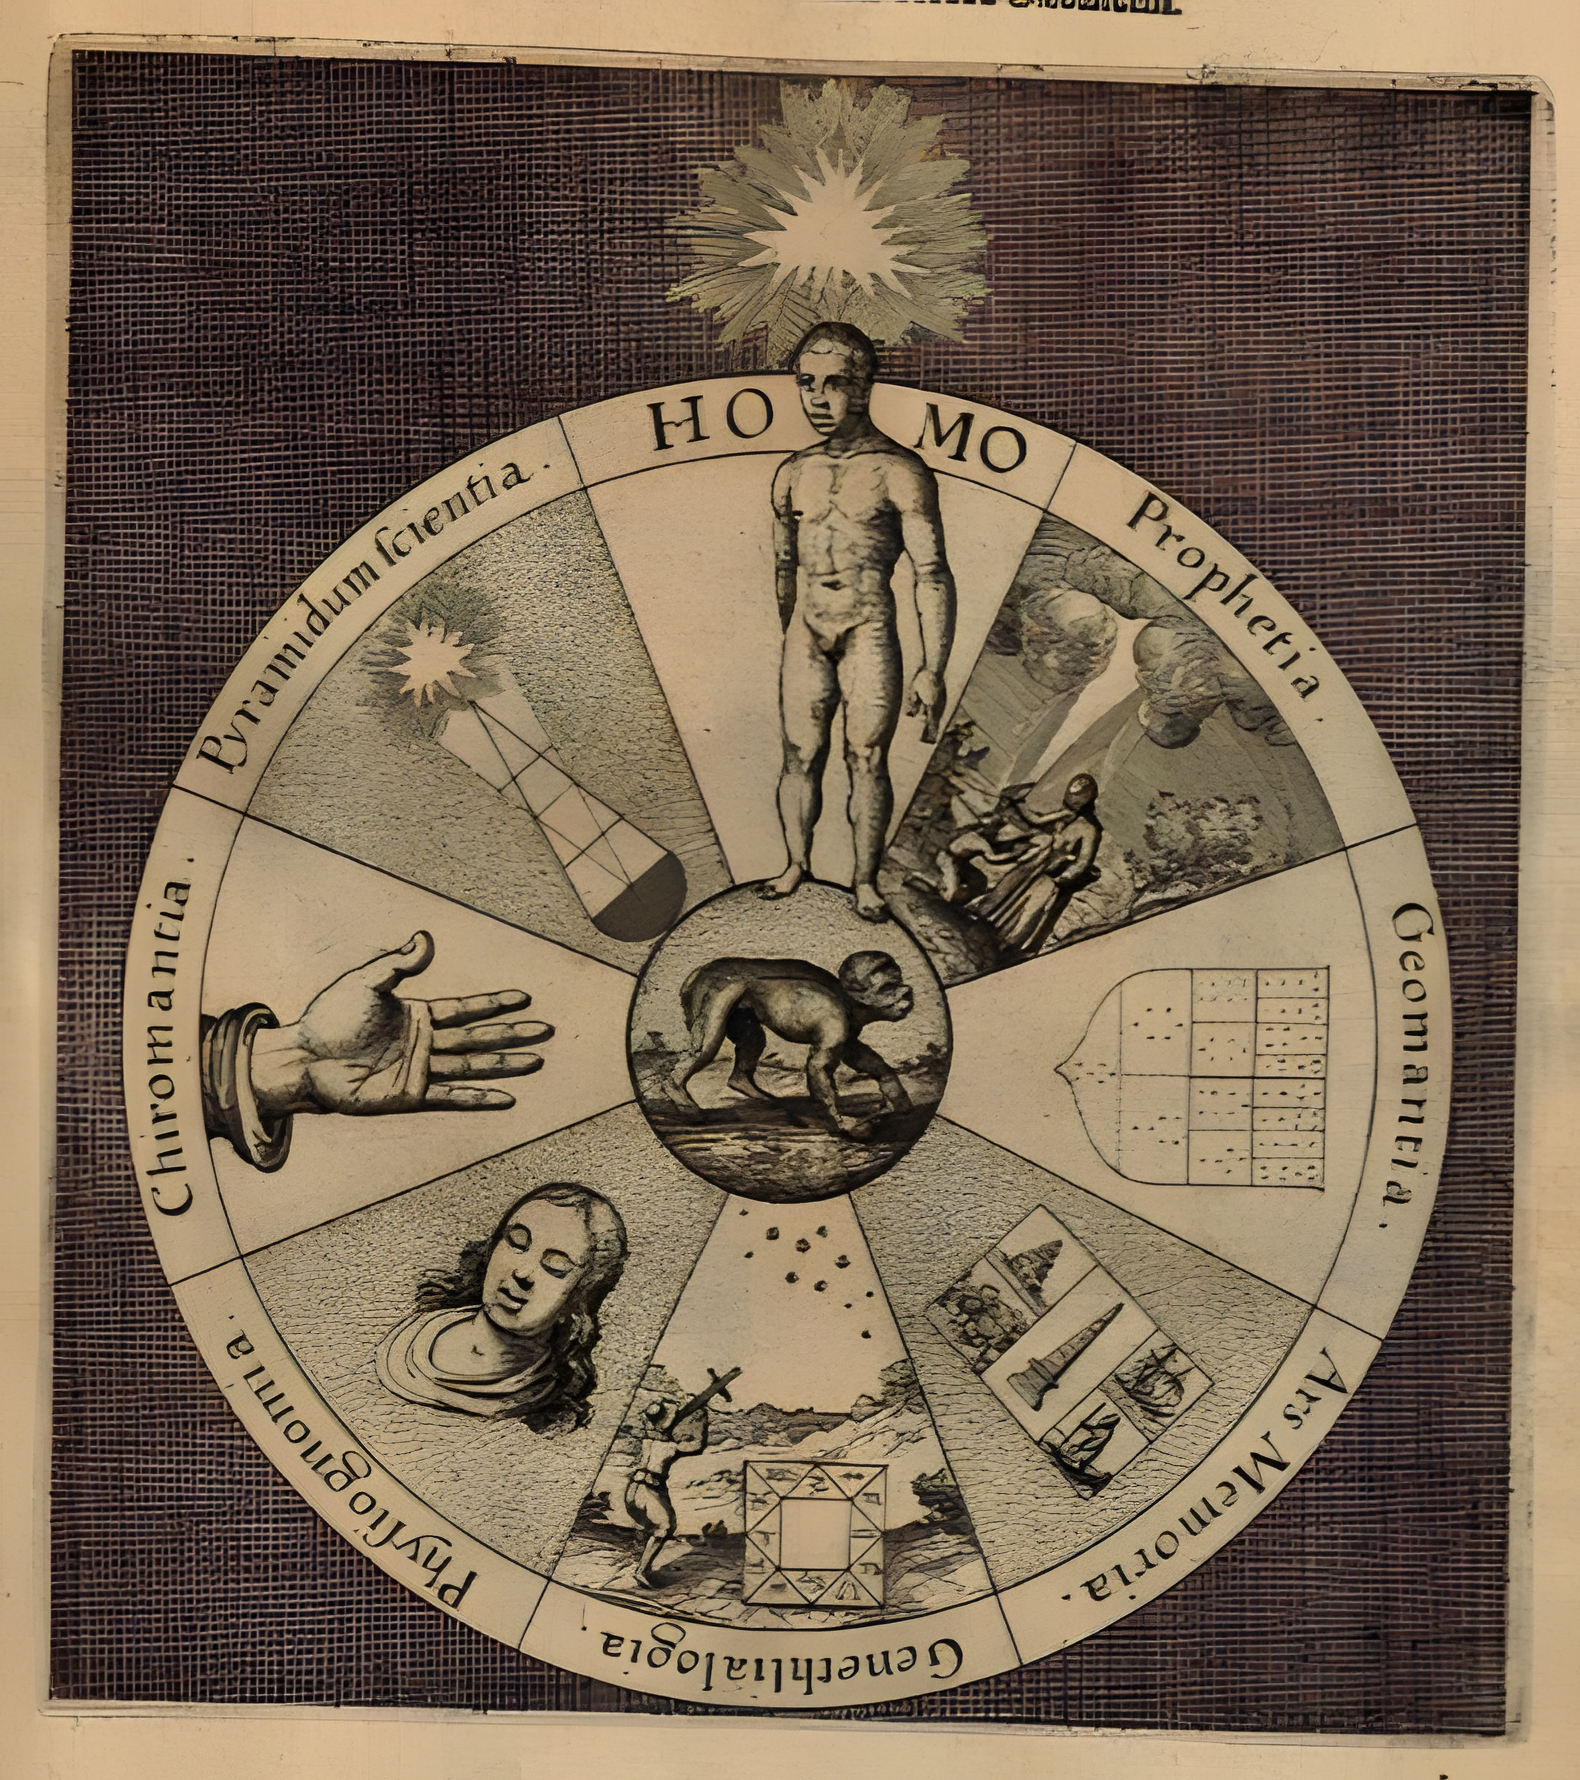
\includegraphics[scale=0.15]{./figures/Pasted image 20240114145552.jpg.png}
\end{center}

Like a good story, our game of imaginary travels can be divided in three main phases, or acts. The \textbf{First Act} is about populating the board with some initial concepts before starting the actual game. This can be done by choosing some main topics beforehand, such as the themes of a conference or the main books of a collection, or through a series of more or less randomised contribution by each player, like the \textbf{Game of 20 Questions} module explained in section \ref{game-of-20-questions}.

The \textbf{Second Act} is the main phase of our game, where players will create connections, quarrel and discuss new concepts on the board. This is done mainly through \textbf{actions associated to dice results} that the players can use to influence the conversation.

The act can be subdivided in \textbf{rounds}, where each player rolls a poll of 6 six-sided dice (D6s) and can keep only four of them. Players can spend dice from their kept poll in exchange for \textbf{actions} to perform, as described in table \ref{action-types}. Notice that a result of 1 or 6 is special, giving additional bonusses:

\begin{itemize}
\item \textbf{1}: The player renounces to an active action in exchange for 
	\begin{itemize}
	\item Gain one coin.
	\item Draw a new \textbf{Magic Item} card from the deck. (optional)
	\item Draw 2 cards from the \textbf{Objective} deck and you \textbf{may} exchange a card in your hand with a newly drawn one. (optional)   
	\end{itemize}
\item \textbf{6}: The player can perform a free action of choice, but at the cost of
	\begin{itemize}
	\item Loose one coin. \footnote{Players can always loose coins: negative treasures are as real as negative numbers!}
	\item Draw an extra \textbf{Objective} from the deck. (optional)
	\item Discard a \textbf{Magic Item} card from their hand. (optional)
	\end{itemize}
\end{itemize}

\begin{table}[h!]
     \begin{center}
     \begin{tabular}{ c  p{3cm}  p{8cm}  }
     \toprule
      Symbol & Name \& dice value & Description \\ 
    \cmidrule(r){1-1}\cmidrule(lr){2-2}\cmidrule(l){3-3}
     \raisebox{-\totalheight}{\includegraphics[width=15mm, height=15mm]{./figures/fluffy-wing.png}}
      & 
      \begin{center}
      \Large{Create \\ 2}
      \end{center}
      & 
      The player can spend their die to:
      \begin{itemize}[topsep=0pt]
      \item Write down a new entity on the board
      \item connect the new concept with a pre-existing one using a property. 
      \item Explain the newly created relationship and entity.
      \end{itemize} \\
      \hline
      \cmidrule(r){1-1}\cmidrule(lr){2-2}\cmidrule(l){3-3}
     \raisebox{-\totalheight}{\includegraphics[width=15mm, height=15mm]{./figures/fox.png}}
      & 
      \begin{center}
      \Large{Manipulate \\ 3}
      \end{center}
      & 
      The player can spend their die to:
      \begin{itemize}[topsep=0pt]
      \item Choose an entity on the board.
      \item Force another player to perform immediately spend a die to perform an action on the chosen entity. 
      \end{itemize} \\
	\hline
      \cmidrule(r){1-1}\cmidrule(lr){2-2}\cmidrule(l){3-3}
     \raisebox{-\totalheight}{\includegraphics[width=15mm, height=15mm]{./figures/classical-knowledge.png}}
      & 
      \begin{center}
      \Large{Advocate \\ 4}
      \end{center}
      & 
      The player can spend their die to:
      \begin{itemize}[topsep=0pt]
      \item Connect two existing entities through a third one, acting as \textbf{qualifier} for the relation.
      \item Connect the three entities with each other forming a triangle of edges.
      \item Explain the newly created relationships.      
       \end{itemize} \\
       \hline
      \cmidrule(r){1-1}\cmidrule(lr){2-2}\cmidrule(l){3-3}
     \raisebox{-\totalheight}{\includegraphics[width=15mm, height=15mm]{./figures/scales.png}}
      & 
      \begin{center}
      \Large{Quarrel \\ 5}
      \end{center}
      & 
      The player can spend their die to:
      \begin{itemize}[topsep=0pt]
      \item Choose an entity on the board.
      \item Choose an opponent.
      \item Choose to talk in favour or against the chosen entity, the opponent must take the other side.
      \item Players have two short rounds each, starting from the player that performed the current action, to convince the rest of the table about their claim. 
      \item The rest of the table vote for the most convincing player.
      \item The winner immediately gets to connect the discussed concept with another one of choice though a property. Furthermore, they get to re-roll one die from their poll.       
       \end{itemize} \\
      \\ \bottomrule
      \end{tabular}
      \caption{Action Types}
      \label{action-types}
      \end{center}
      \end{table}
      
\subsection{Reward and growth}

\begin{center}
\includegraphics[scale=0.45]{./figures/card-game-16thcentury.jpg}
\end{center}



The \textbf{Third Act}, and final one, is a moment for the players at the table to enjoy and reflect about the generated knowledge graph. Take some minutes, and notes, to discuss some interesting relationships between entities that arouse from play and conversation.

\textit{A Shelves Voyage}, as every good games, has a competitive element in it. Competition and reward are powerful tools to increase the motivation of players. We play games to immerse ourselves into an experience, but there is a part of us that just want to beat our fellow players. 

At the end of the game, the player with the highest number of coins wins. To make the game more interesting, we advice to consider using the \textbf{Objectives deck} and \textbf{Support} modules described respectively in section \ref{objective-deck} and \ref{support}.  

\newpage

\section{Modules}

\subsection{The Game of 20 Questions}\label{game-of-20-questions}

\subsection{Magic Items}\label{magic-item-deck}

\subsection{Objectives}\label{objective-deck}

\subsection{Support}\label{support}



\section{Conclusion}


\end{document}

